\section{SimpIL: The language}
\subsection{The basics}
A precise definition of dynamic taint analysis or forward symbolic execution must target a specific language: we use SimpIL, a Simple Intermediate Language. Although the language is simple, it is powerful enough to express typical languages as varied as Java and assembly code. Indeed, the language is representative of internal representations used by compilers for a variety of programming languages. A program in this language consists of a sequence of numbered statements. Statements in our language consist of assignments, assertions, jumps, and conditional jumps.

Expressions are side-effect free, and we use \texttt{$\lozenge$b} to represent typical binary operators, e.g., addition, subtraction, etc. Similarly, \texttt{$\lozenge$u} represents unary operators such as logical negation. The statement \texttt{get\_input(src)} returns input from source src. We use a dot (·) to denote an argument that is ignored, e.g., we will write \texttt{get\_input(·)} when the exact input source is not relevant. For simplicity, we consider only expressions (constants, variables, etc.) that evaluate to 32-bit integer values.

\begin{figure}[h]
	\caption{SimpIL Grammar}
	\centering
	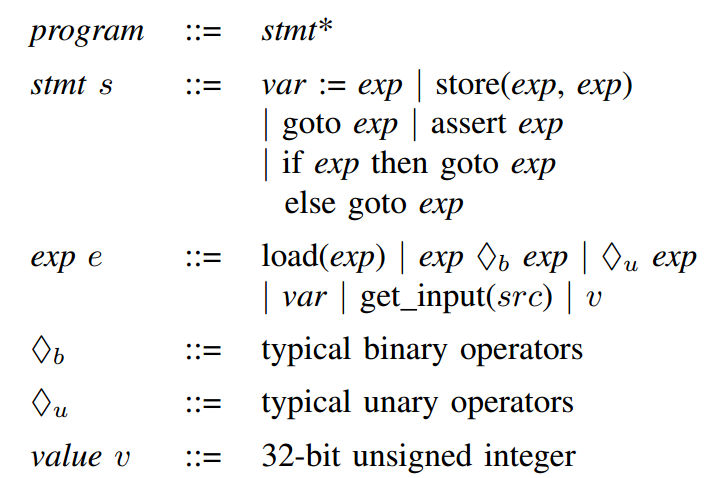
\includegraphics[width=0.7\textwidth]{SimpILBN}
\end{figure}

Because dynamic program analyses are defined in terms of actual program executions, operational semantics also provide a natural way to define a dynamic analysis. Each statement rule is of the form:
\begin{prooftree}
	\AxiomC{computation}
	\UnaryInfC{$\textless$current state$\textgreater$, stmt $\rightarrow$ $\textless$end state$\textgreater$, stmt’}
\end{prooftree}
Rules are deterministic and read bottom to top, left to right. Given a statement, we pattern-match the statement to find the applicable rule.

The execution context is described by five parameters: the list of program statements (\bm{$\sum$}), the current memory state (\bm{$\mu$}), the current value for variables (\bm{$\Delta$}), the program counter (\textbf{\textit{pc}}), and the current statement (\textbf{\textit{i}}). The \bm{$\sum$}, \bm{$\mu$}, and \bm{$\Delta$} contexts are maps. In our evaluation rules, the program context \bm{$\sum$} does not change between transitions. The implication is that our operational semantics do not allow programs with dynamically generated code.